\documentclass[12pt]{article}
\usepackage{graphicx,../lp,amsmath}
% Cross-references for handout numbers.
\usepackage{amsfonts}
%\usepackage{amsthm}
\usepackage{hyperref}
\usepackage{amssymb}
%\usepackage[capitalize]{cleveref}
\usepackage{xcolor}

%\input{handouts}

\newcounter{chapnum}

\newtheorem{definition}{Definition}[chapnum]
\newtheorem{remark}{Remark}[chapnum]
\newtheorem{theorem}{Theorem}[chapnum]
\newtheorem{lemma}[theorem]{Lemma}
\newtheorem{corollary}[theorem]{Corollary}
\newtheorem{proposition}[theorem]{Proposition}
\newtheorem{claim}[theorem]{Claim}
\newtheorem{observation}{Observation}[chapnum]

\renewcommand{\thesection}{\arabic{chapnum}.\arabic{section}}
\renewcommand{\thefigure}{\arabic{chapnum}.\arabic{figure}}


\newenvironment{proof}{\noindent{\bf Proof:} \hspace*{1em}}{
        \hspace*{\fill} $\triangle$ }
\newenvironment{proof_of}[1]{\noindent {\bf Proof of #1:}
        \hspace*{1em} }{\hspace*{\fill} $\triangle$ }
\newenvironment{proof_claim}{\begin{quotation} \noindent}{
        \hspace*{\fill} $\diamond$ \end{quotation}}
\newenvironment{solution}{\noindent{\bf Solution:} \hspace*{1em}}{
        \hspace*{\fill} $\triangle$ }


\newcommand{\R}{{\mathbb R}}
\newcommand{\Z}{{\mathbb Z}}
\newcommand{\Q}{{\mathbb Q}}
\newcommand{\C}{{\mathbb C}}
\newcommand{\N}{{\mathbb N}}
\newcommand{\lin}{\operatorname{lin}}
\newcommand{\aff}{\operatorname{aff}}
\newcommand{\cone}{\operatorname{cone}}
\newcommand{\conv}{\operatorname{conv}}
\newcommand{\vol}{\operatorname{vol}}
\newcommand{\poly}{\operatorname{poly}}




\newcommand{\CF}[1]{{\color{purple}[CF: #1]}}


\newlength{\toppush}
\setlength{\toppush}{2\headheight}
\addtolength{\toppush}{\headsep}

\newcommand{\htitle}[2]{\noindent\vspace*{-\toppush}\newline\parbox{6.5in}
{Massachusetts Institute of Technology \hfill 18.453: Combinatorial Optimization 
\newline
\textbf{Instructor:} Cole Franks \quad \textbf{Notes: }Michel Goemans and Zeb Brady \hfill#2\newline
\mbox{}\hrulefill\mbox{}}\vspace*{1ex}\mbox{}\newline
\begin{center}{\Large\bf #1}\end{center}}

\newcommand{\handout}[2]{\thispagestyle{empty}
 \markboth{ #1 \hfil #2}{ #1 \hfil #2}
 \pagestyle{myheadings}\htitle{#1}{#2}}


\setlength{\oddsidemargin}{0pt}
\setlength{\evensidemargin}{0pt}
\setlength{\textwidth}{6.5in}
\setlength{\topmargin}{0in}
\setlength{\textheight}{8.5in}


\newcounter{exercisenum}
\newcounter{exercisetot}
\setcounter{exercisetot}{0}



\newenvironment{exercises}{
	\begin{list}{{\bf Exercise \arabic{chapnum}-\arabic{exercisenum}. \hspace*{0.5em}}}
	{\setlength{\leftmargin}{0em}
	 \setlength{\rightmargin}{0em}
	 \setlength{\labelwidth}{0em}
	 \setlength{\labelsep}{0em}
	\usecounter{exercisenum}
      \setcounter{exercisenum}{\theexercisetot}}}{\setcounter{exercisetot}{\theexercisenum}\end{list}}


\newenvironment{pseudocode}{
    \begin{list}{}{
        \renewcommand{\makelabel}{$\triangleright$}
        \setlength{\topsep}{0pt}
        \setlength{\leftmargin}{32pt}
        \setlength{\labelwidth}{14pt}
        \setlength{\labelsep}{0mm}
        \setlength{\itemindent}{0mm}
        \setlength{\itemsep}{-3pt}
        \setlength{\itemsep}{0mm}
        \setlength{\parsep}{0pt}%
        \setlength{\listparindent}{0pt}
    }
}
{
    \end{list}
}


\setcounter{chapnum}{2}

\begin{document}

\handout{\arabic{chapnum}. Lecture notes on non-bipartite matching}{\today}

Given a graph $G=(V,E)$, we are interested in finding and
charaterizing the size of a maximum matching. Since we do not assume that
the graph is bipartite, we know that the maximum size of a matching
does not necessarily equal the minimum size of a vertex cover, as is
the case for bipartite graphs (K\"onig's theorem). Indeed, for a
triangle, any matching consists of at most one edge, while we need two
vertices to cover all edges. 

To get an upper bound on the size of any matching $M$, consider any set
$U$ of vertices. If we delete the vertices in $U$ (and all edges
adjacent to it), we delete at most $|U|$ edges of the matching
$M$. Moreover, in the remaining graph $G\setminus U$, we can trivially
upper bound the size of the remaining matching by $\sum_{i=1}^k \lfloor
\frac{|K_i|}{2} \rfloor$, where $K_i$, $i=1,\cdots,k$, are the vertex
sets of the connected components of $G\setminus U$. Therefore, we get
that 
\begin{equation} \label{eq1}
|M| \leq |U| +  \sum_{i=1}^k \left\lfloor
\frac{|K_i|}{2} \right\rfloor.\end{equation}
If we let $o(G\setminus U)$ denote the number of odd components of
$G\setminus U$, we can rewrite (\ref{eq1}) as:
$$ |M| \leq |U| +\frac{|V|-|U|}{2} -\frac{o(G\setminus U)}{2},$$
or
\begin{equation} \label{eq2}
|M| \leq \frac{1}{2} \left( |V| + |U| -o(G\setminus U) \right).
\end{equation}

We will show that we can always find a matching $M$ and a set $U$ for which
we have equality; this gives us the following minmax relation, called
the Tutte-Berge min-max formula:
\begin{theorem}[Tutte-Berge Formula] \label{tutte}
For any graph $G=(V,E)$,  we have 
$$\max_M |M| = \min_{U\subseteq V}
 \frac{1}{2} \left( |V| + |U| -o(G\setminus U) \right),
$$
where $o(G\setminus U)$ is the number of connected components of odd
size of $G\setminus U$.
\end{theorem}

\noindent {\bf Example:} In the graph of Figure \ref{fig-matching}, a
matching of size 8 can be easily found (find it), and its optimality
can be seen from the Tutte-Berge formula. Indeed, for the set
$U=\{2,15,16\}$, we have $o(G\setminus U)=5$ and
$\frac{1}{2}(|V|+|U|-o(G\setminus U))=\frac{1}{2} (18+3-5)=8$. 

\begin{figure}[htbp]
\begin{center}
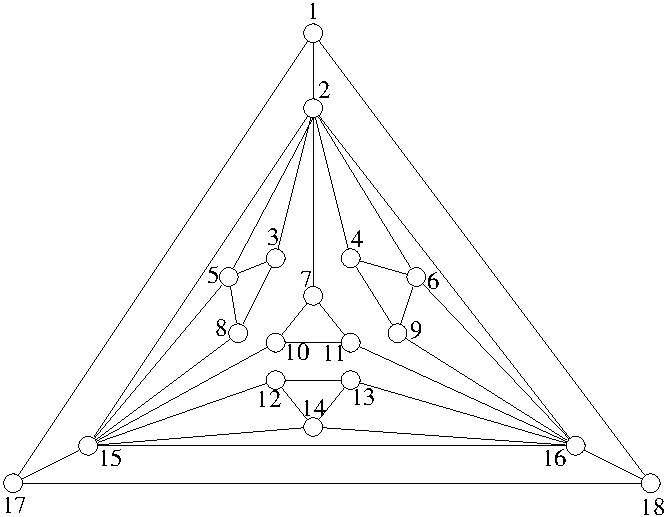
\includegraphics{../figures/matching}

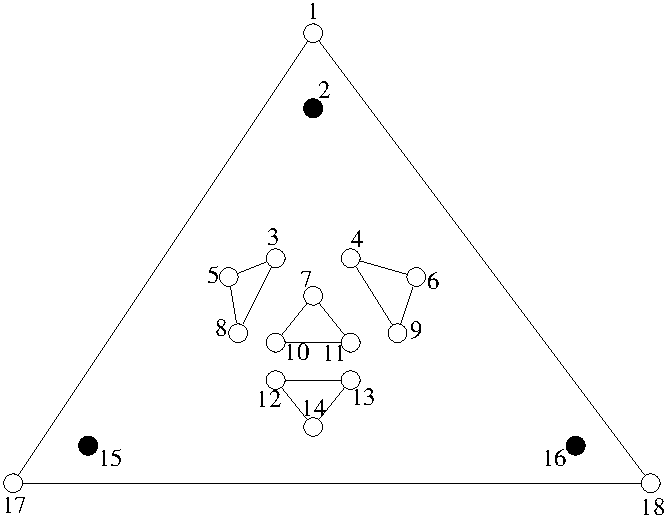
\includegraphics{../figures/matching1}
\end{center}
\caption{\label{fig-matching} Top: graph. Bottom: the removal of
  vertices 2, 15 and 16 gives 5 odd connected components.}
\end{figure}

  
To prove Theorem \ref{tutte}, we will first show an algorithm to find a
maximum matching. This algorithm is due to Edmonds [1965], and is a
pure gem.  As in the case of bipartite matchings (see lecture notes on
bipartite matchings), we will be using augmenting paths. Indeed,
Theorem 1.2 of the bipartite matching notes still holds in the
non-bipartite setting; a matching $M$ is maximum if and only if there
is no augmenting path with respect to it. The difficulty here is to
find the augmenting path or decide that no such path exists. We could
try to start from the set $X$ of exposed (unmatched) vertices for $M$,
and whenever we are at a vertex $u$ and see an edge $(u,v)\notin M$
followed by an edge $(v,w)$ in $M$, we could put a directed edge from
$u$ to $w$ and move to $w$. If we get to a vertex that's adjacent to
an exposed vertex (i.e. in $X$), it seems we have found an augmenting
path, see Figure \ref{fig-augm}. 

\begin{figure}[htbp]
\begin{center}
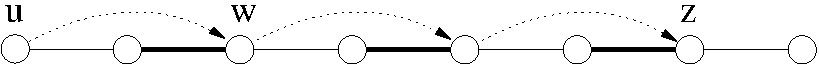
\includegraphics{../figures/augpath}
\end{center}
\caption{\label{fig-augm} An augmenting path. Thick edges are in the
  matching. The path is found by starting from the exposed vertex $u$
  and following the dotted lines until a vertex (here $z$) adjacent to
  an exposed vertex is found. }
\end{figure}

This is not necessarily the case, as the vertices of this `path' may
not be distinct. In this case we have found a so-called  {\it
  flower}, see Figure \ref{flower}. This flower does not contain an
augmenting path. More formally, a {\it flower} consists of an even
alternating path $P$ from an exposed vertex $u$ to a vertex $v$,
called the {\it stem}, and an odd cycle containing $v$ in which the
edges alternate between in and out of the matching except for the two
edges incident to $v$; this odd cycle is called a {\it blossom}.    

\begin{figure}[htbp]
%\vspace{40pt}
\begin{center}
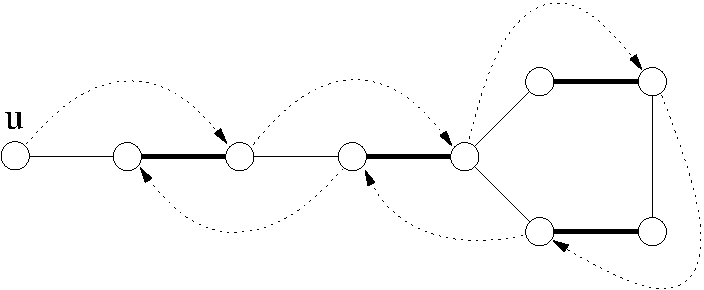
\includegraphics{../figures/flower3}
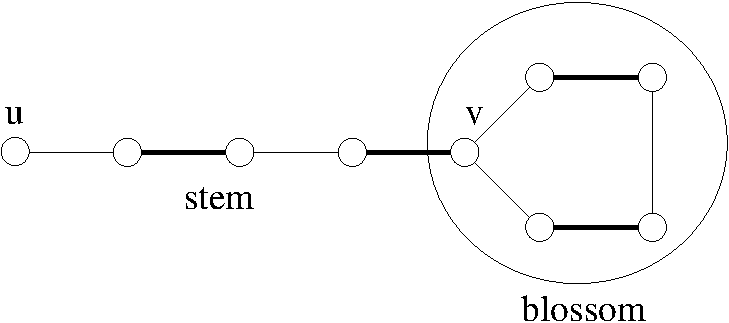
\includegraphics{../figures/flower2}
\end{center}
\caption{\label{flower} A flower. The thick edges are those of the
  matching. Top: Our dotted path starting at an exposed vertex $u$ and
  ending at a neighbor of an exposed vertex does not correspond to an
  augmenting path. }
%\vspace{8pt}
\end{figure}

The algorithm will either find an augmenting path or a flower or show
that no such items exist; in this latter case, the matching is maximum
and the algorithm stops. If it finds an augmenting path then the
matching is augmented and the algorithm continues with this new
matching. If a flower is found, we
create a new graph $G/B$ in which we shrink the blossom $B$ into a single vertex
$b$; any edge $(u,v)$ in $G$ with $u\notin B$ and $v\in B$ is replaced
by an edge $(u,b)$ in $G/B$, all edges within $B$ disappear and all
edges within $V\setminus B$ are kept. Notice that we have also a
matching $M/B$ in this new graph (obtained by simply deleting all
edges of $M$ within $B$), and that the sizes of $M$ and $M/B$ differ
by exactly $\frac{|B|-1}{2}$ (as we deleted so many edges of the
matching within $B$). We use the following crucial theorem.

\begin{theorem} \label{thm:unshrink}
Let $B$ be a blossom with respect to $M$. 
Then M is a maximum size matching in $G$ if and only
if $M/B$ is a maximum size matching in $G/B$.
\end{theorem}

Moreover, the proof is algorithmic: If we have a bigger matching in
$G/B$ than $M/B$ then we also can find a bigger matching in $G$ than
$M$. This shows that, assuming we have an algorithm to find either a flower or alternating path when it exists, we have a \textbf{recursive algorithm} that takes in a matching and outputs a larger one: when we find a flower with blossom $B$, use the results of the algorithm recursively applied to $G/B$ to increase the size of $M$.\\
 
\begin{proof_of}{\ref{thm:unshrink}}
To prove the theorem, we can assume that the flower with blossom $B$ has an empty stem $P$. If it is not the case, we can consider the matching $M\bigtriangleup P=(M\setminus P)\cup (P\setminus M)$ for which we have a flower with blossom $B$ and empty stem. Proving the theorem for $M\bigtriangleup P$ also proves it for $M$ as $(M\bigtriangleup P)/B =(M/B)\bigtriangleup P$ and taking symmetric differences with an even alternating path does not change the cardinality of a matching. Now we begin the proof.


($\Longrightarrow$)  Suppose $N$ is a matching in $G/B$ larger
than $M/B$.  Pulling $N$ back to a set of edges in $G$,
it is incident to at most one vertex of $B$.  Expand this to a
matching $N^+$ in $G$ by adjoining $\frac{1}{2}(|B|-1)$ edges
to match every other vertex in $B$.  Then $|N^+|$ exceeds $|M|$
by the same amount that $|N|$ exceeds $|M/B|$.

($\Longleftarrow$) By contradiction. If $M$ is not of maximum size in
$G$ then it has an augmenting path $P$ between exposed vertices $u$
and $v$. As $B$ has only one exposed vertex (recall that its stem is empty), we can assume that $u\notin B$. Let $w$ be the first vertex of $P$ which belongs to $B$, or let $w=v$ if $B$ and $P$ share no vertices. Let $Q$ be the part of $P$ from $u$ to $w$. Notice that, after
shrinking $B$, $Q$ remains an augmenting path for $M/B$ (since either $w=b$, which is
exposed in $G/B$, or $w = v \not\in B$ which remains exposed in $G/B$). This means that $M/B$ is not maximum either, and we
have reached a contradiction.
\end{proof_of}

Note that Theorem \ref{thm:unshrink} does {\it not} say
that if we find a maximum matching $M^*$ in $G/B$ then simply adding
$\frac{|B|-1}{2}$ edges from within $B$ to $M^*$ to get $\hat{M}$ will
lead to a {\it maximum} matching in $G$. Indeed, this is not true. 

\begin{exercises}
\item
Give an example of a graph $G$, a matching $M$ and a blossom $B$ for
$M$ such that a maximum matching $M^*$ in $G/B$ does not lead to a
maximum matching in $G$. Explain why this does not contradict Theorem
\ref{thm:unshrink}. 
\end{exercises}

\begin{figure}[htbp]
\begin{center}
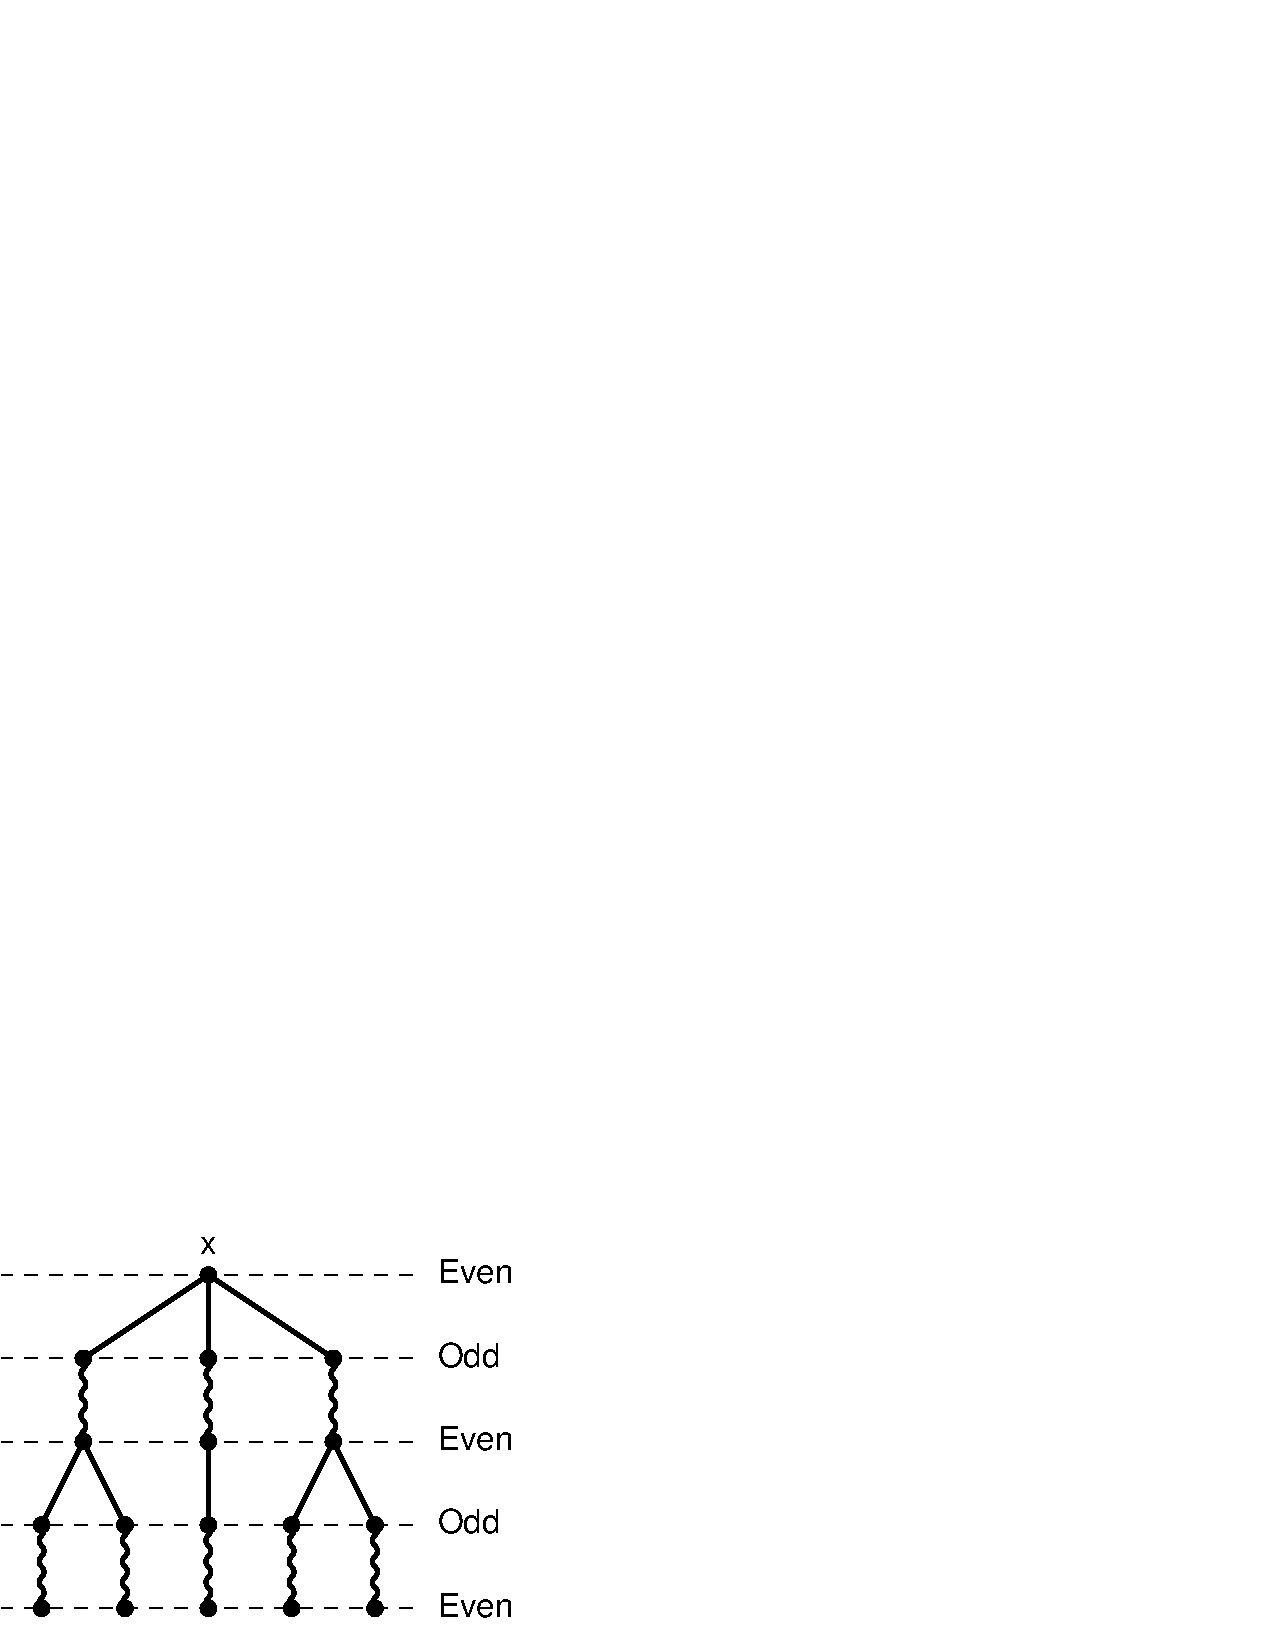
\includegraphics{../figures/evenodd}
\end{center}
\caption{\label{alttree} An alternating tree. The squiggly edges are the
matching edges.}
\end{figure}

\paragraph{Edmonds' Algorithm.}
We now describe the algorithm in full, including the subroutine for finding an augmenting path or flower. Start with some arbitrary matching $M$, and repeat the following until termination.\\
 
\noindent \boxed{\textbf{Plant Forest:}} Given a matching $M$, To find either an augmenting path or a flower, we proceed as
follows. We label all exposed vertices to be {\sc Even}, and keep all the
other vertices unlabelled at this point. As we proceed, we will be
labelling more vertices to be {\sc Even} as well as labelling some
vertices to be {\sc Odd}. We maintain also an {\it alternating forest} ---
a graph in which each connected component is a tree made up of edges
alternating between being in and out of the matching. Right now each {\sc Even} vertex is its own singleton tree in the forest, or ``seed," if you like :).
 \begin{itemize}

\item\boxed{\textbf{Grow Forest:}}
Given an alternating tree and a partial labelling, we process the
{\sc Even} vertices one at a time. Say we are currently processing $u$,
and consider the edges adjacent to $u$. There are several
possibilities:
\begin{enumerate}
\item
If there is an edge $(u,v)$ with $v$ unlabelled, we label $v$
as {\sc Odd}. As $v$ cannot be exposed (as otherwise it would have been
already {\sc Even}), we label its ``mate'' $w$ (i.e. $(v,w)$ is an edge of
the matching) as {\sc Even}. ($w$ was not previously labelled as we always
simultaneously label the two endpoints of a matched edge.) 
We have extended the alternating tree we are
building (see Figure \ref{alttree}).
\item
If there is an edge $(u,v)$ with $v$ labelled {\sc Even} and $v$ belongs
to another alternating tree than $u$ does, we have found an
augmenting path (just traverse the 2 alternating trees from $u$ and
$v$ up to their roots) and augment the matching along it, and start again
from this new, larger matching. The two subpaths from $u$ and from $v$
to their roots span disjoint sets of vertices, and therefore their
union together with $(u,v)$ indeed form a valid augmenting path. Augment this path in the current graph to obtain a matching with one more edge, and then obtain a matching with one more edge in the original graph by unshrinking any blossoms we've shrunk and using Theorem \ref{thm:unshrink}. The new matching may not be optimal, so we return to \boxed{\textbf{Plant Forest}} in the original graph with the new matching. 
\item
If there is an edge $(u,v)$ with $v$ labelled {\sc Even} and $v$ belongs
to the same alternating tree as $u$ does, then the two subpaths from
$u$ and $v$ to their common (exposed) root $x$ together with $(u,v)$
form a flower. We shrink the blossom $B$ into a vertex $b$. Observe that we can keep our
labelling unchanged, provided we let the new vertex $b$ be labelled
{\sc Even}. Return to \boxed{\textbf{Grow Forest}} with the smaller graph $G/B$ with and the matching $M/B$ with the same labeling but with the new vertex $b$ labelled {\sc Even}.
%(and this may result in further shrinkings) and when the algorithm
%terminates, we use Theorem \ref{thm:unshrink} to expand it to a larger
%matching in the original graph. This larger matching is not
%necessarily optimal (see the remark after Theorem \ref{thm:unshrink})
%and we repeat the process to find either an augmenting path or a
%flower with respect to the current matching. 
\end{enumerate}
If none of the possibilities hold, \textbf{Terminate} and output the matching obtained by unshrinking the blossoms as described in the proof of Theorem \ref{thm:unshrink}.
\end{itemize}

\paragraph{Correctness.} Now suppose that none of these possibilities
apply any more for any of the {\sc Even} vertices. Then we claim that we
have found a maximum matching $M'$ in the current graph $G'=(V',E')$
(which was obtained from our original graph $G$ by performing several
shrinkings of blossoms $B_1, B_2, \cdots, B_k$ in
succession). To show this, consider $U=\textsc{Odd}$ and consider the upper
bound \ref{eq2} for $G'$. As there are no edges between {\sc Even}
vertices (otherwise 2.~or 3.~above would apply) and no edges between
an {\sc Even} vertex and an unlabelled vertex (otherwise 1.~would apply),
we have that each {\sc Even} vertex is an (odd-sized) connected component by
itself in $G'\setminus \textsc{Odd}$. Thus $o(G'\setminus \textsc{Odd})=|\textsc{Even}|$. Also,
we have that $|M'|=|\textsc{Odd}| + \frac{1}{2} (|V'|-|\textsc{Odd}|-|\textsc{Even}|)$, the
second term coming from the fact that all unlabelled vertices are
matched. Thus, $$\frac{1}{2}(|V'|+|\textsc{Odd}|-o(G'\setminus
\textsc{Odd}))=\frac{1}{2}(|V'|+|\textsc{Odd}|-|\textsc{Even}|)=|M'|,$$ and this shows that our
matching $M'$ is maximum for $G'$. Applying repeatedly Theorem
\ref{thm:unshrink}, we get that the algorithm constructs a maximum
matching in $G$.

\paragraph{Running Time.} The algorithm will perform at most $n/2$
augmentations (of the matching) where $n=|V|$. Between two
augmentations, it will shrink a blossom at most $n/2$ times, as each
shrinking reduces the number of vertices by at least 2. The time it
takes to construct the alternating tree is at most $O(m)$ where
$m=|E|$, and so the total time is $O(n^2m)$. 

\paragraph{Correctness of Tutte-Berge Formula.} We can now prove
Theorem \ref{tutte}. As we have argued the Tutte-Berge formula holds
for the graph obtained at the end of the algorithm. Assume we have
performed $k$ blossom shrinkings, and let $G_i=(V_i,E_i)$ be the
graph obtained after shrinking blossoms $B_1, \cdots, B_i$, and let
$M_i$ be the corresponding matching; the index $i=0$ corresponds to
the original graph. For the final graph $G_k=(V_k,E_k)$, we have seen
that the Tutte-Berge formula holds since 
$$|M_k|=\frac{1}{2} \left( |V_k|+|U|-o(G_k\setminus U) \right),$$
where $U=\textsc{Odd}$, and that each {\sc Even} vertex corresponds to an odd
connected component of $G_k\setminus U$. Now, 
let's see what happens when we unshrink blossoms, one at a time, and
let's proceed by backward induction. Suppose 
we unshrink blossom $B_i$ to go from graph $G_i$ to $G_{i-1}$. First
notice that  $|V_{i-1}|=|V_i|+|B_i|-1$ and
$|M_{i-1}|=|M_i|+\frac{1}{2} (|B_i|-1)$. Also, as we unshrink blossom
$B_i$, we add an even number of vertices (namely $|B_i|-1$) to one of the connected
components of $G_i\setminus U$ because the shrunk blossoms $b_i$ are labeled {\sc Even} (see Step 3 of the algorithm). Therefore, we do not change the
number of odd (or even) connected components. Thus, $o(G_i\setminus
U)=o(G_{i-1}\setminus U)$. Thus, as we replace $i$ with $i-1$, both
the right-hand-side and left-hand-side of 
$$|M_i|=\frac{1}{2} \left( |V_i|+|U|-o(G_i\setminus U) \right)$$
increase by precisely $\frac{1}{2}(|B_i|-1)$.  
Thus, by backward induction, we can show
that for every $j=0,\cdots,k$, we have
$$|M_j|=\frac{1}{2} \left( |V_j|+|U|-o(G_j\setminus U) \right),$$
and the Tutte-Berge formula holds for the original graph (for
$j=0$). This proves Theorem \ref{tutte}.

The Tutte-Berge formula implies that a graph has a perfect matching if
and only if for every set $U$ the number of odd connected components
of $G\setminus U$ is at most $|U|$. This is known as {\bf Tutte's
  matching theorem.}  

\begin{theorem}[Tutte's matching theorem]
$G$ has a perfect matching if and only if, for all $U\subseteq V$, we
have $o(G\setminus U)\leq |U|$. 
\end{theorem}

\subsection*{Exercises}
\begin{exercises}
\item
Let $G=(V,E)$ be any graph. Given a set
$S\subseteq V$, suppose that there exists a matching $M$ covering $S$
(i.e. $S$ is a subset of the matched vertices in $M$). Prove that
there exists a {\it maximum} matching $M^*$ covering $S$ as well. 

%%%%%%%%%%%%%%
\item \label{ex2-3}
Let $U$ be any minimizer in the Tutte-Berge formula. Let $K_1,
  \cdots, K_k$ be the connected components of $G\setminus U$.  Show
  that, for {\it any} maximum matching $M$, we must have that
\begin{enumerate}
\item
$M$ contains exactly $\lfloor \frac{|K_i|}{2}\rfloor$ edges from
$G[K_i]$ (the subgraph of $G$ induced by the vertices in
$K_i$), i.e. $G[K_i]$ is perfectly matched for the even components $K_i$ and
near-perfectly matched for the odd components. 
\item
Each vertex $u\in U$ is matched to a vertex $v$ in an odd component
$K_i$ of $G\setminus U$.
\item
the only unmatched vertices must be in odd components $K_i$ of
$G\setminus U$.  
\end{enumerate}  

%%%%%%%%%%%
\item
Could there be several minimizers $U$ in the Tutte-Berge formula?
Either give an example with several sets $U$ achieving the minimum, or
prove that the set $U$ is unique.  

%%%%%%%%%%%%%%%%%%
\item % from 4 Bills book, page 134, ex 5.6
Given a graph $G=(V,E)$, an {\it inessential} vertex is a vertex $v$
such that there exists a {\it maximum} matching of $G$ not covering
$v$. Let $B$ be the set of all inessential vertices in $G$ (e.g., if
$G$ has a perfect matching then $B=\emptyset$). Let $C$ denote the set
of vertices not in $B$ but adjacent to at least one vertex in $B$
(thus, if $B=\emptyset$ then $C=\emptyset$). Let $D=V\setminus (B\cup
C)$. The triple $\{B, C, D\}$ is called the Edmonds-Gallai partition
of $G$. Show that $U=C$ is a minimizer in the Tutte-Berge formula. (In
particular, this means that in the Tutte-Berge formula we can assume
that $U$ is such that the union of the odd connected components of
$G\setminus U$ is precisely the set of inessential vertices.)



%%%%%%%%%%%%%
\item  Show that any 3-regular 2-edge-connected graph $G=(V,E)$ (not
  necessarily bipartite)
 has a perfect matching.  (A 2-edge-connected graph has at least 2 edges in
  every cutset; a cutset being the edges between $S$ and $V\setminus
  S$ for some vertex set $S$.) 

%%%%%%%%%%%%%%%
\item
A graph $G=(V,E)$ is said to be {\it factor-critical} if, for all
$v\in V$, we have that $G\setminus \{v\}$ contains a perfect
matching. In parts (a) and (b) below, $G$ is a factor-critical graph.
\begin{enumerate}
\item
Let $U$ be {\it any} minimizer in the
Tutte-Berge formula for $G$. Prove that $U=\emptyset$. (Hint: see
Exercise \thechapnum-\ref{ex2-3}.)
\item
Deduce that when Edmonds algorithm terminates the final graph
(obtained from $G$ by shrinking blossoms) must be a single vertex. 
\item
Given a graph $H=(V,E)$, an {\it ear} is a path
$v_0-v_1-v_2-\cdots-v_k$ whose endpoints ($v_0$ and $v_k$) are in
$V$ and whose internal vertices ($v_i$ for $1\leq i \leq k-1$) are not
in $V$. We allow that $v_0$ be equal to $v_k$, in which case the path
would reduce to a cycle. Adding the ear to $H$ creates a new graph on
$V\cup\{v_1,\cdots,v_{k-1}\}$. The trivial case when $k=1$ (a `trivial' ear) simply
means adding an edge to $H$. An ear is called {\it odd} if $k$ is odd, and
even otherwise; for example, a trivial ear is odd. 
 \begin{enumerate}
\item 
Let $G$ be a graph that can be constructed by starting from an odd
cycle and repeatedly adding odd ears. Prove that $G$ is
factor-critical. 
\item 
Prove the converse that any factor-critical graph can be built by starting from an
odd cycle and repeatedly adding odd ears.
\end{enumerate}
 \end{enumerate}
\end{exercises}



\end{document}
